% A DAE stage solves differential and algebraic values together.
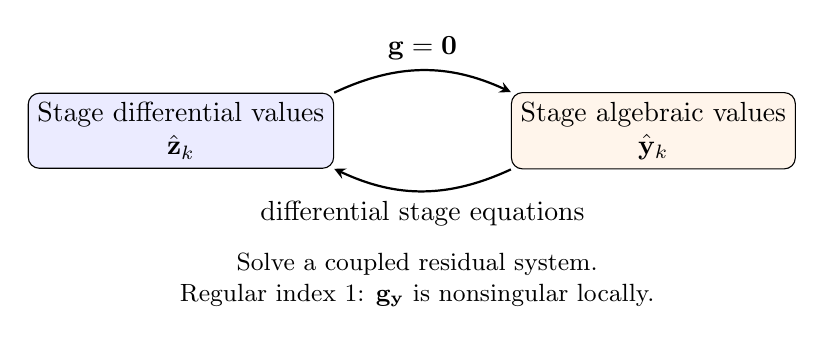
\begin{tikzpicture}[>=stealth,font=\normalsize,box/.style={draw,rounded corners,align=center,minimum height=.9cm}]
\node[box,fill=blue!8](z)at(0,0){Stage differential values\\$\hat{\mathbf z}_k$};
\node[box,fill=orange!8](y)at(6,0){Stage algebraic values\\$\hat{\mathbf y}_k$};
\draw[->,thick](z.north east)to[bend left=25]node[above]{$\mathbf g=\mathbf0$}(y.north west);
\draw[->,thick](y.south west)to[bend left=25]node[below]{differential stage equations}(z.south east);
\node[font=\small,align=center]at(3,-1.9){Solve a coupled residual system.\\Regular index~1: $\mathbf g_{\mathbf y}$ is nonsingular locally.};
\end{tikzpicture}
